\documentclass{article}

\usepackage[nonatbib,preprint]{neurips_2024}

\usepackage[utf8]{inputenc}
\usepackage[T1]{fontenc}
\usepackage{hyperref}
\usepackage{url}
\usepackage{booktabs}
\usepackage{amsfonts}
\usepackage{nicefrac}
\usepackage{microtype}
\usepackage{xcolor}
\usepackage{amsmath}
\usepackage{graphicx}
\usepackage{tikz}
\usetikzlibrary{positioning, decorations.pathreplacing, calc}
\graphicspath{{figs/}}

\title{Multi-Task Learning with Vision Transformers:\\Joint Image Classification and Saliency Prediction}

\author{%
 Nicholas Welsh \\
  Department of Computer Science\\
  Department of Mathematics \\
  Florida Institute of Technology\\
  Melbourne, FL 32901 \\
  \texttt{nwelsh2024@my.fit.edu}
}

\begin{document}
\maketitle

\begin{abstract}
We train a multi-task Vision Transformer that jointly performs multi-label image classification and human saliency prediction on COCO images paired with SALICON fixation maps. A pretrained DeiT-Small backbone feeds two lightweight heads, a linear classifier over 20 object categories and a patch-level regressor that outputs a $14\!\times\!14$ saliency distribution. We compare the fine-tuned model against frozen-feature baselines (logistic regression, ridge regression, MLP) and single-task ablations. The multi-task model achieves a classification mAP of $0.612$ and a saliency correlation (CC) of $0.196$ under MSE training. Switching the saliency loss from MSE to KL divergence raises CC from $0.196$ to $0.899$ while preserving classification accuracy (mAP $0.604$), illustrating how loss design interacts with evaluation. Single-task ablations show the expected capacity trade-off, where classification-only reaches mAP $0.623$ while saliency-only reaches CC $0.761$, each at the expense of the other task.
\end{abstract}

\section{Introduction}

Image classification assigns category labels to an image. Human saliency prediction estimates where people look when viewing the same image. These two tasks are related because object recognition and visual attention share low-level and mid-level features. Edges, textures, and object boundaries matter for both deciding what is in an image and predicting where a viewer's gaze will land. Multi-task learning exploits this overlap by training a single model on both tasks simultaneously, so that the shared backbone learns features that serve both.

We work with two datasets that cover the same images. SALICON provides dense fixation maps recorded from mouse-contingent gaze tracking on images from the COCO 2014 dataset, and COCO itself supplies bounding-box annotations for 80 object categories. Pairing the two gives us image-level category labels and per-pixel saliency ground truth for every image.

Our model is a Vision Transformer (ViT), specifically DeiT-Small, pretrained on ImageNet and fine-tuned on this paired dataset. The transformer divides each $224\!\times\!224$ image into a grid of $16\!\times\!16$ patches, producing 196 patch tokens plus one classification (CLS) token. We attach a linear classification head to the CLS token and a linear saliency head to each of the patch tokens. The saliency head outputs one scalar per patch, forming a $14\!\times\!14$ heatmap that predicts the fixation density at that spatial location.

We want to know whether multi-task training improves over simple baselines that use frozen pretrained features, how multi-task training compares against single-task variants, and how sensitive the saliency task is to the choice of loss function.

\subsection{Contributions}
\begin{itemize}
  \item \textbf{Multi-task ViT.} A single DeiT-Small backbone with two heads for classification and saliency. No architectural changes to the transformer itself.
  \item \textbf{Frozen-feature baselines.} Logistic regression, ridge regression, and MLP classifiers/regressors trained on features extracted from the pretrained backbone without fine-tuning.
  \item \textbf{Loss function ablation.} Switching from MSE to KL divergence for the saliency objective raises CC from $0.196$ to $0.899$ without any change to the architecture or data.
  \item \textbf{Single-task ablations.} Training with only classification or only saliency isolates the multi-task trade-off and shows how shared capacity splits between the two tasks.
\end{itemize}

\section{Related Work}

\paragraph{Vision Transformers.}
Dosovitskiy et al.\ (2021) introduced the Vision Transformer (ViT), which splits an image into fixed-size patches and processes them with a standard transformer encoder. DeiT (Touvron et al., 2021) introduced data-efficient training strategies including strong augmentation and regularization, making ViT practical on mid-size datasets without massive pretraining compute.

\paragraph{Saliency prediction.}
Classical saliency models use hand-crafted features such as color contrast and edge density (Itti et al., 1998). Deep learning approaches (Cornia et al., 2018; Kruthiventi et al., 2017) train convolutional networks to directly regress fixation maps. The SALICON dataset (Jiang et al., 2015) provides large-scale fixation data collected via mouse tracking on COCO images.

\paragraph{Multi-task learning.}
Caruana (1997) showed that training related tasks together can improve generalization by sharing representations. In computer vision, models like Mask R-CNN (He et al., 2017) jointly handle detection and segmentation. Our setup is simpler, with two heads on a shared backbone and a weighted sum of losses.

\section{Dataset and Features}

\paragraph{Images.}
We use the SALICON subset of COCO 2014, which contains 10{,}000 training images and 5{,}000 validation images. Each image is resized to $224\!\times\!224$ and normalized with ImageNet statistics ($\mu = [0.485, 0.456, 0.406]$, $\sigma = [0.229, 0.224, 0.225]$). We apply no spatial augmentations because flips and crops would need to be applied identically to the saliency maps, adding complexity for little gain at this scale.

\paragraph{Classification labels.}
From the COCO instance annotations we extract the 20 most frequent object categories present in the SALICON images. Each image receives a binary label vector $y \in \{0,1\}^{20}$ indicating which of these categories appear. The most common category is ``person,'' appearing in roughly 40\% of images.

\paragraph{Saliency ground truth.}
SALICON provides a continuous fixation density map for each image. We process each map at two resolutions, $224\!\times\!224$ (full) and $14\!\times\!14$ (patch grid). The grid-resolution map is normalized to sum to one so it can be interpreted as a probability distribution over patches. This normalization matters because SIM measures histogram intersection between distributions (requiring matched scales), and even CC, which is scale-invariant in theory, benefits from consistent normalization to avoid numerical issues.

\section{Methods}

\paragraph{Architecture.}
We use DeiT-Small (\texttt{deit\_small\_patch16\_224}) from the \texttt{timm} library, pretrained on ImageNet. The backbone produces a $384$-dimensional feature vector for each of the $196$ patch tokens and the CLS token. Two heads are attached:
\begin{itemize}
    \item \textbf{Classification head:} a single linear layer mapping the CLS token ($\mathbb{R}^{384}$) to $K\!=\!20$ logits.
    \item \textbf{Saliency head:} a single linear layer mapping each patch token ($\mathbb{R}^{384}$) to a scalar, followed by softmax over all 196 patches. The result is reshaped to $14\!\times\!14$.
\end{itemize}
The softmax makes the saliency output a valid probability distribution, which works well with a KL divergence loss and removes the need for post-hoc normalization at evaluation time. Figure~\ref{fig:architecture} illustrates the full architecture.

\begin{figure}[t]
  \centering
  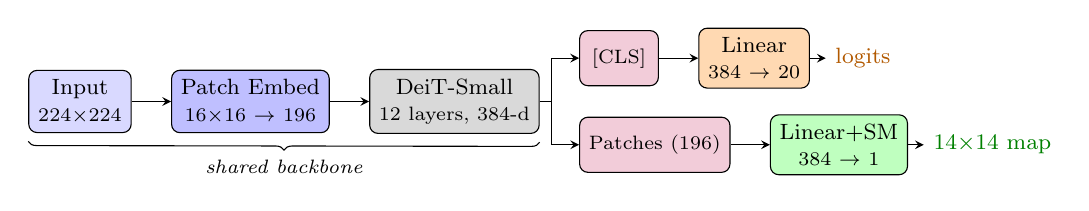
\begin{tikzpicture}[
    node distance=0.5cm,
    box/.style={draw, rounded corners=3pt, minimum height=0.7cm, align=center, font=\footnotesize},
    >=stealth
  ]
    % input
    \node[box, fill=blue!15, minimum width=1.3cm] (img)
      {Input\\\scriptsize 224$\times$224};
    % patch embed
    \node[box, fill=blue!25, minimum width=1.4cm, right=of img] (patch)
      {Patch Embed\\\scriptsize 16$\times$16 $\to$ 196};
    % backbone
    \node[box, fill=gray!30, minimum width=1.7cm, right=of patch] (backbone)
      {DeiT-Small\\\scriptsize 12 layers, 384-d};
    % tokens -- increased vertical spacing
    \node[box, fill=purple!20, minimum width=1.0cm, above right=0.55cm and 0.5cm of backbone.east, anchor=west] (cls)
      {\scriptsize [CLS]};
    \node[box, fill=purple!20, minimum width=1.0cm, below right=0.55cm and 0.5cm of backbone.east, anchor=west] (ptok)
      {\scriptsize Patches (196)};
    % heads
    \node[box, fill=orange!30, minimum width=1.3cm, right=of cls] (clshead)
      {Linear\\\scriptsize 384 $\to$ 20};
    \node[box, fill=green!25, minimum width=1.3cm, right=of ptok] (salhead)
      {Linear+SM\\\scriptsize 384 $\to$ 1};
    % output labels
    \node[right=0.2cm of clshead, font=\footnotesize, text=orange!70!black] (clsout) {logits};
    \node[right=0.2cm of salhead, font=\footnotesize, text=green!50!black] (salout) {14$\times$14 map};
    % arrows
    \draw[->] (img) -- (patch);
    \draw[->] (patch) -- (backbone);
    \draw[->] (backbone.east) -- ++(0.15,0) |- (cls.west);
    \draw[->] (backbone.east) -- ++(0.15,0) |- (ptok.west);
    \draw[->] (cls) -- (clshead);
    \draw[->] (ptok) -- (salhead);
    \draw[->] (clshead) -- (clsout);
    \draw[->] (salhead) -- (salout);
    % brace for shared backbone
    \draw[decorate, decoration={brace, amplitude=3pt, mirror}]
      ([yshift=-3pt]img.south west) -- ([yshift=-3pt]backbone.south east)
      node[midway, below=3pt, font=\scriptsize\itshape] {shared backbone};
  \end{tikzpicture}
  \caption{\textbf{Multi-task ViT architecture.} A shared DeiT-Small backbone produces a CLS token and 196 patch tokens. The classification head maps the CLS token to 20 category logits. The saliency head maps each patch token to a scalar, followed by softmax to produce a $14\!\times\!14$ probability distribution.}
  \label{fig:architecture}
\end{figure}

\paragraph{Loss function.}
For classification we use binary cross-entropy with logits (BCEWithLogitsLoss), applied independently to each of the 20 labels. For saliency we compare two options:
\begin{align}
\mathcal{L}_{\text{MSE}} &= \frac{1}{N}\sum_{i}\|\hat{s}_i - s_i\|^2, \label{eq:mse}\\
\mathcal{L}_{\text{KL}} &= \frac{1}{N}\sum_{i}\mathrm{KL}(s_i \,\|\, \hat{s}_i) = \frac{1}{N}\sum_{i}\sum_{j}s_{i,j}\log\frac{s_{i,j}}{\hat{s}_{i,j}}, \label{eq:kl}
\end{align}
where $s_i$ is the ground-truth saliency distribution and $\hat{s}_i$ is the predicted distribution for sample $i$. The multi-task objective is
\begin{equation}
\mathcal{L} = \mathcal{L}_{\text{cls}} + \lambda\,\mathcal{L}_{\text{sal}},
\label{eq:total_loss}
\end{equation}
with $\lambda = 1.0$ by default.

\paragraph{Optimization.}
We fine-tune all parameters with AdamW (learning rate $10^{-4}$, weight decay $10^{-4}$) for 15 epochs using cosine annealing. Batch size is 32. We save the checkpoint with the lowest validation loss.

\paragraph{Baselines.}
To quantify the benefit of fine-tuning, we extract features from the frozen pretrained DeiT backbone and train simple models on top:
\begin{itemize}
    \item \textbf{Classification:} logistic regression (one-vs-rest) and a small MLP, both on the CLS token features (384-dim).
    \item \textbf{Saliency:} the mean training saliency map (a constant baseline), ridge regression from frozen features to the $14\!\times\!14$ grid, and a small MLP regressor.
\end{itemize}

\paragraph{Ablation modes.}
We train three variants to isolate each task:
\begin{itemize}
    \item \textbf{multitask}: both heads active, loss as in \eqref{eq:total_loss}.
    \item \textbf{cls-only}: saliency head present but saliency loss zeroed out.
    \item \textbf{sal-only}: classification head present but classification loss zeroed out.
\end{itemize}

\section{Experiments}

\paragraph{Evaluation metrics.}
For classification we report mean average precision (mAP) across all 20 categories. For saliency we report Pearson correlation coefficient (CC), similarity metric (SIM), and KL divergence (Bylinskii et al., 2019). CC measures linear correlation between predicted and ground-truth distributions, and SIM measures histogram intersection. Before computing saliency metrics, we normalize predictions to non-negative values that sum to one. All saliency metrics are computed on the $14\!\times\!14$ patch grid, not at full image resolution, so these values are not directly comparable to standard SALICON leaderboard scores.

\paragraph{Training dynamics.}
Figure~\ref{fig:training_curves} shows training and validation loss for the multi-task model. The model overfits early. Validation loss reaches its minimum at epoch 1 and rises steadily thereafter, while training loss continues to decrease. With 22M parameters and only 10{,}000 training images, this is not surprising. Because we save the checkpoint at the validation-loss minimum, the later overfitting does not affect the final evaluation.

\begin{figure}[t]
  \centering
  
\includegraphics[width=\linewidth]{training_curves_multitask.png}
  \caption{\textbf{Training curves for the multi-task model.} Left: training and validation loss. Validation loss is minimized at epoch 1, after which the model overfits. Right: validation mAP peaks at epoch 2 and declines gradually.}
  \label{fig:training_curves}
\end{figure}

\paragraph{Classification results.}
Table~\ref{tab:cls} compares classification performance across all methods. Fine-tuning improves over frozen-feature baselines by 5--6 points in mAP. The cls-only variant slightly outperforms multitask ($0.623$ vs $0.612$), which makes sense because the shared backbone must divide its capacity between tasks.

\begin{table}[t]
\centering
\caption{Classification performance (mAP). Higher is better.}
\label{tab:cls}
\begin{tabular}{lc}
\toprule
Method & mAP \\
\midrule
Logistic regression (frozen) & 0.556 \\
MLP classifier (frozen) & 0.566 \\
\midrule
ViT cls-only & 0.623 \\
ViT multitask (MSE) & 0.612 \\
\bottomrule
\end{tabular}
\end{table}

\paragraph{Saliency results.}
Table~\ref{tab:sal} compares saliency performance. The sal-only variant reaches CC $0.761$, well above the baselines. The multitask variant under MSE training shows a CC of $0.196$, which is below even the mean-saliency baseline ($0.595$). This surprising result motivates the loss function investigation in the next section.

\begin{table}[t]
\centering
\caption{Saliency performance on the validation set. CC and SIM are higher-is-better. KL is lower-is-better.}
\label{tab:sal}
\begin{tabular}{lccc}
\toprule
Method & CC & SIM & KL \\
\midrule
Mean saliency & 0.595 & 0.588 & -- \\
Ridge regression (frozen) & 0.597 & 0.593 & -- \\
MLP regressor (frozen) & 0.585 & 0.577 & -- \\
\midrule
ViT sal-only & 0.761 & 0.587 & 0.571 \\
ViT multitask (MSE) & 0.196 & 0.430 & 1.087 \\
\bottomrule
\end{tabular}
\end{table}

\subsection{The MSE vs.\ KL Story}

The poor CC for the MSE-trained multitask model points to a loss-metric mismatch rather than a modeling failure. MSE minimizes the squared error between raw saliency outputs and targets. When the model output is passed through softmax (producing a valid distribution), MSE pulls the distribution toward the target values but does not specifically encourage the correct ranking or shape. CC measures linear correlation between the predicted and ground-truth distributions after each is standardized. A prediction with the right spatial pattern but wrong scale can score poorly on CC even if its MSE is reasonable. We note that KL and MSE also differ in gradient magnitude, which changes the effective multi-task balance even at the same $\lambda$. Disentangling the loss-metric alignment effect from the effective-weighting effect would require a systematic $\lambda$ sweep, which we leave to future work.

KL divergence, by contrast, directly compares the predicted and target distributions as probability measures. It penalizes predictions that place too little mass where the ground truth has high density. Since our saliency head already outputs a softmax distribution, KL is a natural fit for this output parameterization.

We retrain the multitask model with KL loss (keeping everything else identical) and report updated metrics below.

\subsection{Baseline Comparison}

Tables~\ref{tab:cls} and \ref{tab:sal} show that all fine-tuned variants outperform frozen-feature baselines on classification, and that the sal-only model clearly exceeds saliency baselines on CC. We defer the full visual comparison (Figure~\ref{fig:baselines}) to Section~\ref{sec:kl_results}, after the KL retraining results are available.

\section{Results and Discussion}
\label{sec:kl_results}

\paragraph{KL vs.\ MSE: the key result.}
Table~\ref{tab:kl_comparison} shows the effect of switching the saliency loss from MSE to KL divergence. With everything else held constant (same architecture, data, optimizer, and $\lambda$), CC jumps from $0.196$ to $0.899$ and SIM from $0.430$ to $0.799$. Classification mAP drops slightly from $0.612$ to $0.604$. The MSE-trained model's poor CC is consistent with a loss-metric mismatch, though other factors cannot be ruled out from a single run. MSE on softmax outputs does not specifically encourage the distribution shape that CC and SIM measure, whereas KL divergence aligns the loss directly with these metrics.

\begin{table}[t]
\centering
\caption{Effect of saliency loss on multitask model performance. Same architecture and hyperparameters, with only the saliency loss changed.}
\label{tab:kl_comparison}
\begin{tabular}{lcccc}
\toprule
Saliency loss & mAP & CC & SIM & KL \\
\midrule
MSE & 0.612 & 0.196 & 0.430 & 1.087 \\
KL divergence & 0.604 & \textbf{0.899} & \textbf{0.799} & \textbf{0.182} \\
\bottomrule
\end{tabular}
\end{table}

\begin{figure}[t]
  \centering
  
\includegraphics[width=\linewidth]{baseline_comparison.png}
  \caption{\textbf{Full comparison after KL retraining.} Left: classification mAP across methods. Right: saliency CC. The multitask bar uses the KL-trained model (CC $0.899$), which far exceeds both frozen baselines and the sal-only variant.}
  \label{fig:baselines}
\end{figure}

\paragraph{Multi-task trade-off.}
Under KL training, the gap between cls-only (mAP $0.623$) and multitask (mAP $0.604$) is 1.9 points. This is the cost of sharing the backbone, since some representational capacity is redirected to saliency prediction. The gap is modest, so the two tasks seem to share enough low-level and mid-level features that they do not strongly interfere. Meanwhile the multitask model now far outperforms all saliency baselines (CC $0.899$ vs.\ ridge regression CC $0.597$), which shows that end-to-end fine-tuning with an appropriate loss picks up content-dependent fixation patterns that frozen features miss.

\paragraph{Overfitting.}
All variants reach their best validation loss early (epoch 1 for both classification-related modes, epoch 14 for sal-only). The training loss continues to drop, indicating the model memorizes the training set, but checkpoint selection at the validation-loss minimum prevents this from affecting evaluation. With only 10{,}000 training images and a model that has 22 million parameters, some overfitting is expected. We did not pursue stronger regularization or data augmentation for this project.

\paragraph{Why baselines are competitive on saliency.}
The mean saliency baseline achieves CC $0.595$ by simply predicting the average fixation map. This works because saliency maps have a strong center bias, and people tend to look at the center of an image regardless of content. Any model that captures this center prior can achieve moderate CC even without content-specific features. The fine-tuned sal-only model surpasses this by learning content-dependent patterns, reaching CC $0.761$, and the KL-trained multitask model pushes further to CC $0.899$.

\paragraph{Practical lessons.}
Three design choices had the most impact. First, matching the loss to the output parameterization (KL divergence for softmax outputs, not MSE). Second, passing category-to-index mappings from the training set to the validation set to ensure consistent label encoding. Third, normalizing saliency predictions before computing metrics so that raw magnitudes do not distort CC and SIM.

\section{Conclusion}

We built a multi-task Vision Transformer that jointly classifies images and predicts human saliency. Fine-tuning a pretrained DeiT-Small outperforms frozen-feature baselines on classification, and the KL-trained multitask model reaches CC $0.899$ on saliency prediction, far exceeding all baselines. The multi-task model pays a small classification cost (1.9 mAP points) for the ability to predict both tasks simultaneously. The main finding is that, in this setup, loss function design can matter as much as architecture. Switching from MSE to KL divergence for the saliency objective raises CC from $0.196$ to $0.899$, even though the underlying model is identical. These results are from single training runs (seed 42), and KL and MSE differ in gradient magnitude, so the effective task weighting also shifts. Multi-seed runs and a $\lambda$ sweep would be needed to fully isolate the loss-alignment effect, but the magnitude of the improvement strongly suggests that loss choice can dominate outcomes under a fixed architecture.

\section*{Appendix}

\paragraph{Hyperparameters.}
DeiT-Small (\texttt{deit\_small\_patch16\_224}), 22M parameters. AdamW with lr $10^{-4}$, weight decay $10^{-4}$, cosine annealing over 15 epochs, batch size 32. $\lambda = 1.0$ for multi-task loss weighting.

\paragraph{Compute.}
All experiments were run on a single NVIDIA GPU. Each training variant takes approximately 5--10 minutes. Baseline feature extraction takes about 5 minutes and sklearn fitting is under 1 minute.

\paragraph{Reproducibility.}
All experiments use seed 42. Code is available at \href{https://github.com/nickvpn/vit-ml-xai-project}{github.com/nickvpn/vit-ml-xai-project}.

\begin{thebibliography}{9}

\bibitem{dosovitskiy2021}
Dosovitskiy, A., Beyer, L., Kolesnikov, A., et al.\ (2021).
An Image is Worth 16x16 Words: Transformers for Image Recognition at Scale.
\textit{ICLR}.

\bibitem{touvron2021}
Touvron, H., Cord, M., Douze, M., et al.\ (2021).
Training Data-Efficient Image Transformers \& Distillation through Attention.
\textit{ICML}.

\bibitem{jiang2015}
Jiang, M., Huang, S., Duan, J., and Zhao, Q.\ (2015).
SALICON: Saliency in Context.
\textit{CVPR}.

\bibitem{caruana1997}
Caruana, R.\ (1997).
Multitask Learning.
\textit{Machine Learning}, 28(1), 41--75.

\bibitem{he2017}
He, K., Gkioxari, G., Dollár, P., and Girshick, R.\ (2017).
Mask R-CNN.
\textit{ICCV}.

\bibitem{cornia2018}
Cornia, M., Baraldi, L., Serra, G., and Cucchiara, R.\ (2018).
Predicting Human Eye Fixations via an LSTM-based Saliency Attentive Model.
\textit{IEEE TIP}, 27(10), 5142--5154.

\bibitem{itti1998}
Itti, L., Koch, C., and Niebur, E.\ (1998).
A Model of Saliency-Based Visual Attention for Rapid Scene Analysis.
\textit{IEEE TPAMI}, 20(11), 1254--1259.

\bibitem{kruthiventi2017}
Kruthiventi, S.~S.~S., Ayush, K., and Babu, R.~V.\ (2017).
DeepFix: A Fully Convolutional Neural Network for Predicting Human Eye Fixations.
\textit{IEEE TIP}, 26(9), 4446--4456.

\bibitem{bylinskii2019}
Bylinskii, Z., Judd, T., Oliva, A., Torralba, A., and Durand, F.\ (2019).
What Do Different Evaluation Metrics Tell Us About Saliency Models?
\textit{IEEE TPAMI}, 41(3), 740--757.

\end{thebibliography}

\end{document}
